\documentclass[10pt]{article}
\usepackage{spconf}
\usepackage{amsmath}
\usepackage[dvips,pdftex]{graphicx}
\usepackage{named}
\usepackage[dvips,pdftex]{hyperref}
\usepackage{subfigure}
\usepackage{array}

\title{Enhanced Particle Swarm Optimization In Sketch Recognition}
\twoauthors
{Maha El Meseery\sthanks{Corresponding Author}, Mahmoud Fakhr El Din}
	{Signals Processing Group \\ Computers and Systems Department \\
  Electronic Research Institute\\Cairo, Egypt\\
	melmeseery@eri.sci.eg, mafakhr@mcit.gov.eg}
  {Tarek abouldahab} {Cairo Metro Company \\
  Ministry of transport \\Cairo, Egypt\\ heshoaboda@hotmail.com}
 

\begin{document}
\maketitle
 \begin{abstract}
%This study 

Sketches and drawings are widely used as a simple method of expressing thought and designs. The goal of this paper is to improve our sketch recognition system by using an enhanced particle swarm optimization algorithm. The enhanced Particle Swarm Optimization (EPSO) is based on the perturbation of the particle velocity is used to optimally segment the strokes the user draws into meaningful geometric primitives.  These geometric primitives are grouped to formulate symbols which are further identified using a Support Vector Machines (SVM) classifier. Experiments were conducted on the benchmark dataset of simple presentation (Hs-DS) symbols. Results show that that the enhanced particle swarm optimization improves the final recognition accuracy. 

\end{abstract}
\pagenumbering{arabic}
 \section{Introduction}

The field of symbol recognition has gained interest in the last few years. Scientists generally and engineers specifically express thoughts and designs using sketches. Engineers use sketches to exchange designs as a natural method of communication rather than writing or speaking. Design engineers need a powerful computer based system with symbol recognition to help them design, manipulate and store sketches more effectively than using only papers. Increasing the interaction between computers and users in sketch and CAD systems has been the reason for the emerging of a few advanced sketch recognition systems. Sketch recognition is the process of identifying user strokes into meaningful symbols that can be further used.  

Sketch recognition is divided into three main steps preprocessing, segmentation and symbol recognition. The preprocessing phase captures user input stroke points and collects basic information about the stroke then proceeds to remove noise and compute basic statistical and geometrical information. In segmentation phase, the strokes are divided into a set of simple geometrical primitives or segments. In the third phase, sketch recognition, strokes and segments are clustered to formulate symbols that can be recognized by a classifier system.

This paper modifies the sketch recognition system presented in \cite{mypaper}, to use enhanced particle swarm algorithm (EPSO) to optimally segment user's strokes. As in the Original system the users can draw symbols using any number of strokes in any order they like. The system segments each stroke using two different EPSO algorithms. Segmentation is based on dividing the digital curve into polygon\cite{PolygonApproximationPSO}. To handle complex strokes, our system uses a second segmentation EPSO algorithm to segment strokes into a set of lines and circular arcs. After segmentation, a symbol features vector composed of different statistical, geometrical and spatial features is deduced. The final classification step, SVM classifier uses the computed feature vector to classify the segments into one of the previously trained classes. 

The remaining of the paper is as following; Section \ref{sec:ParticleSwarmAlgorithm} describes the Basic particle swarm algorithm in details.  Enhanced Particle Swarm Algorithm is described in Section \ref{sec:EnhancedSwarmAlgorithm}. Section \ref{Sysdisc} provide details on preprocessing, segmentation and recognition process. Section \ref{sec:Experiments} describes the experiments that were preformed. We conclude in Section \ref{ConclusionandFutureWork}.
 

\section{Basic Particle Swarm Optimization}
\label{sec:ParticleSwarmAlgorithm}

 Particle Swarm Algorithm\cite{PSOFirst}is a population based stochastic search where each solution is simulated as a  particle that flies around in a multidimensional search space. A fitness function is used to evaluate the goodness of each particle in solution space. But unlike evolutionarily algorithm the new population is the PSO is influenced by the social cooperation of the particle rather than survival to the fittest. Each particle saves a history of the best location in the swarm and its own best location.  At the end each iteration, the particles moves to a new location based on the global best location and it own history of best location. This use of previous particle locations gives PSO advantage over Evolutionary algorithms where no similar information is used.

 The \textit{Basic Particle Swarm Algorithm (PSO)} represents each solution with a $N$ dimension particle from the solution space \cite{PSOFirst}. Each particle moves with a direction and velocity $v_{ij}$ based on equations \ref{eq:Swarm1} \& \ref{eq:Swarm}.


\begin{equation}
%\[
p_{ij}=p_{ij}+v_{ij},
%\
\label{eq:Swarm1}
\end{equation}
 
where $p_{ij}$ represent the $j$th dimension in the $i$th particle and $v_{ij}$ is the velocity of the $j$th dimension in the $i$th particle.

 \begin{equation}
v_{ij}  = v_{ij} \omega + c_1 r_1 (lbest_{ij}  - p_{ij} ) + c_2 r_2 (gbest_{ij}  - p_{ij} ),
\label{eq:Swarm}
\end{equation}
 where $\omega$ is the inertia weight parameter which controls the tradeoff between exploration and exploitation,  $lbest_{ij}$ is the local best particle, $gbest_{ij}$ is the global best particle, $r_1$ \& $r_2$ are random variables and $c_1$ \& $c_2$ are the swarm acceleration parameters.  
 
 After each iteration the global best $g_{best}$ particle and the agent local best particle $l_{best}$are evaluated based on the maximum fitness functions of all particles in the solution space. The solution is found after achieving a specific number of iteration or after an error threshold is achieved.

\section{Enhanced Particle Swarm}
\label{sec:EnhancedSwarmAlgorithm}
In the above basic PSO, the velocity update is based on three terms an inertia term, local cognitive ($l_{best}$) term and global cognitive ($g_{best}$)term. The particle local cognitive term is associated with the particle own history without consideration of other swarm particles locations and histories which leads to a lake of diversity and sub optimum solutions. Therefore, we are trying to add more social influence in the particle movement by using the weighted difference of the position vectors of any other two distinct particles randomly chosen from the swarm to modify the local cognitive term. The modified term adds social behavior of other particle and keeps diversity while searching for the global optimum. The new social cognitive term of the particle is shifted to the new location only if it yields a fitness value better than obtained using the standard PSO\cite{stockPaper}.

This modification is done as follows:-
  \begin{enumerate}
\item For each particle $p_{i}$ in the swarm two other distinct particles, $p_L$ and $p_M$ are selected randomly where $i\neq L\neq M$. The difference between their positional coordinates $p_{d}$ is taken as a difference vector in equation \ref{eqmod}.
 \begin{equation}
 \label{eqmod}
 p_{dj}= p_{Lj}-p_{Mj} 
 \end{equation}
where $p_{dj}$ represent the $j$th dimension in the difference vector and $p_{Lj}$ represent the $j$th dimension in the $L$th particle. 

Then the associated velocity vector of particle $p_{i}$ is updated according to this difference vector as in equation \ref{eq:mod1}. In essence the local cognitive term of the velocity update formula in \ref{eq:Swarm} is replaced with the vector differential operator $p_d$ to produce some additional exploration capability.
 \begin{equation}
 v^{T}_{ij}  = v_{ij} \omega + c_1 r_1 (p_{dj}) + c_2 r_2 (gbest_{ij}  - p_{ij} ),
 \label{eq:mod1}
 \end{equation}
\item The new trial position $p^{T}_{ij}$ is created by adding the updated velocity $v^{T}_{ij}$ in Eq. \ref{eq:mod1}.
  \begin{equation}
 \label{eq:mod2}
p^{T}_{ij}=p_{ij}+ v^{T}_{ij} ,
 \end{equation}
\item The new position $p^{T}_{ij}$ is used to generate the new trial objective fitness function value $fitness(p^{T})$. The fitness value is calculated based on this new trial position vector and the particle is shifted to this trial position if the trial objective function is better than the original objective function associated with standard PSO. Thus the target particle is relocated using the following equation (Eq. \ref{eq:objective}) 
  \begin{equation}
 \label{eq:objective}
p^{new}_{ij}\Leftarrow 
\{
\begin{array}{c} 
 p^{T}_{ij} \quad \quad if\quad fitness(p^{T})> fitness(p^{old})  \\
 p_{ij} \quad \quad Otherwise\quad  
\end{array}\}
 \end{equation}
 where $fitness(p^{T})$ is the objective fitness value of the new trail position $ p^{T}$ and  $fitness(p^{old})$is the objective fitness value of the new basic position $ p{i}$ computed by equation \ref{eq:Swarm1}. 
   \end{enumerate}

\section{System Discribtion  }\label{Sysdisc}
%\label{sec:application}
The modified swarm algorithm is used to improve the performance of the sketch recognition system in \cite{mypaper}. The sketch recognitions system is divided into three main steps 1) preprocessing, 2) segmentation and 3) Recognition. The following section provides a detailed description of each step. The main block of the system remains the same but their is some modification in the segmentation algorithm to improve its efficiency. The main modification is using Enhanced Particle swarm algorithm instead of Basic Particle swarm algorithms. Other modifications are explained in the details in the next sections.  
\subsection{Preprocessing}
\label{Prepross}
 Speed and time difference information were widely used in sketch understanding systems \cite{earlyprocess}. It was noted that time difference provides more distinct maxima than the speed information. Agar \cite{polygonfeedback31} mentions that the pointing device (i.e. the mouse) sampling rate is the reason for this phenomenon. 
 In the presented system, we computed time difference, direction, speed and curvature of each point along a stroke. The speed is calculated as $v=\Delta s/\Delta t$ where $t$ is the time difference between two points and $s$ is the length between them. The direction $d$ is calculated as the angle between two vectors and curvature is considered as the change in direction with respect to length i.e. $c= \Delta d/\Delta s$. Dominant points are characterized by lower speed values and higher curvature and direction values.
  
After the system computes all the speed, time difference and curvature information it proceeds to detect the points with low velocity and high curvatures. Using simple differentiation to detect local extreme points resulted in false points due to the non smooth curves. Hence, the system adopted a process presented by \cite{earlyprocess}, where the mean of the curve is calculated. Then a threshold \textit{th} is used to separate the curve into regions $Region_i$; each region $Region_i$ is defined as a range of points, where the curve values are either above or below the threshold \textit{th}. Those regions are further processed to find the maximum point $Max(Region_i)$ of each region $Region_i$. The stroke points $p_i(x,y)$ that correspond to those maximum values are labeled as \textit{possible dominant points} $P_{pd}$. The system repeats this process for curvature, time difference and speed information. All the points labeled as possible dominant points $P_{pd}$ are saved into a single array. Figure \ref{fig:LabelsPPD} shows the particles labeled as Possible dominant point $P_{pd}$ by the preprocessing, it is noticed the redundancy of some $P_{pd}$ points. % (as shown are redundant)
\subsection{Segmentation}
\label{seg}
In the segmentation stage the input stroke is divided into a set of primitives. As shown in Figure \ref{fig:segblock} first an attempt is made to fit the stroke points into a curve or an ellipse using a minimum square error fitting algorithm \cite{ellipsefit}. The ellipse fitting step helps to prevent the system from over segmenting the stroke into multiple lines or curves if the input stroke is an ellipse. If the stroke proved to be an ellipse arc then the segmentation process ends and the system proceeds to the next step. Otherwise, the stroke is passed to two further segmentation algorithms that divide the stroke to either lines or lines and curves. After two different segmentations are generated, the system chooses the segmentation with the minimum error. The following sections describe in details the ellipse detection algorithm and the two segmentation algorithms used to divide the stroke. 
 \begin{figure}
	\centering
		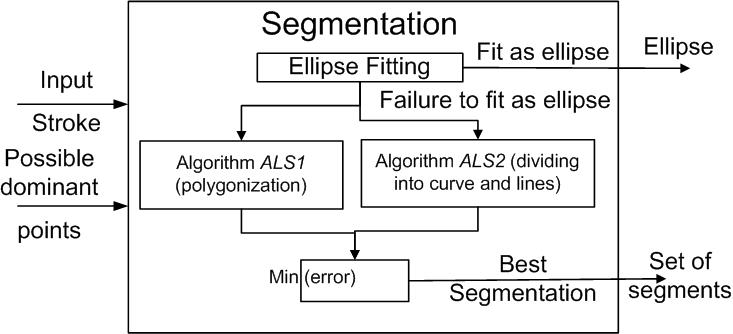
\includegraphics[scale=0.48]{blockSmall.jpg}
	\caption{Segmentation Block}
	\label{fig:segblock}
\end{figure}
\subsection{Ellipse fitting}

This process tries to fit the stroke points into an ellipse arc; it starts with computing the center of the stroke bounding box. The bounding box center point is used as the first estimation of the center of the ellipse. The axes of the ellipse are estimated as the $width/2$ and $height/2$ of the stroke bounding box where $width$ is width and $height$ is height of the bonding box. The least square fitting algorithm \cite{chernov} is used to minimize the fitting error of the ellipse Equation (\ref{eq:circleFit})  

\begin{equation}
E = \sum\limits_{i = 0}^N {\frac{{(x_i - x_0 )}}{{a^2 }}^2  + \frac{{(y_i - y_0 )}}{{b^2 }}^2  - 1} 
\label{eq:circleFit}
\end{equation}

 where $N$ is number of points in the stroke, $a,b$ are the length of ellipse axes, $x_0$ \& $y_0$ are the coordinates of the center point, $x_i$ \& $y_i$ are the coordinates of point $i$ in the stroke. A list of new values for $x_0$ , $y_0$ ,$a$ and $b$ are generated randomly from the older values with small increments after each loop.  After few iteration, the final fit error of the estimated ellipse is reported. A modification to the system in \cite{mypaper} is trying to add another measure to compute the efficiency of the final estimated ellipse. Equation \ref{eq:circleError} ensures that the drawn percentage of ellipse is considered. This eliminates fitting a line into very large ellipse but leaves small ellipses to be fitted as a partial or full ellipse. 

 \begin{equation}
eff= (P_{percent}/E)
\label{eq:circleError}
\end{equation}
 \begin{equation}
P_{percent}  = L_{stroke} /P_{ellipse} 
\label{eq:ErrorArea}
\end{equation}
where $E$ is the error computed by Equation(\ref{eq:circleFit}), $L_{stroke}$ total length of stroke and $P_{ellipse} $ is the perimeter of the estimated ellipse. If $eff$ is more than threshold $th_{Ellipse}$\footnote{By trial and error best threshold found was $th_{Ellipse}=0.2$} then the stroke is segmented as an ellipse otherwise the system proceeds to the next step. 

\subsection{Non ellipse fitting algorithm}
\label{subsubsec:Discreteparticleswarmalgorithm}
\begin{figure}
	\centering
	
	 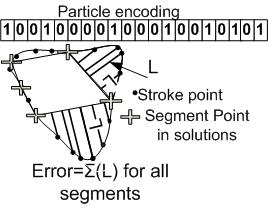
\includegraphics[scale=0.7]{pso1.jpg}			
	\caption{DPSO algorithm encoding}
	\label{fig:pso1}
\end{figure}
Two DPSO algorithms are used to generate different segmentations for each stroke the user draws. For each segmentation generated, an error is evaluated. The segmentation with the minimum error value is chosen as the best stroke segmentation (Figure \ref{fig:segblock}). The problem definition is the same in both algorithms but they differ in the method they use to compute fitness and error functions. 
\begin{description}
	\item[ Problem definition:] The input stroke $S$  with $N$ points can be represented by set $S = \left\{ {x_1 ,x_2  \ldots x_N }\right\}$ where $x_i$ is the location of the point $i$. The swarm algorithms consist of $M$ agents which are represented by the set $A = \left\{ {P_i \left| {i = 1,2 \cdots M} \right.} \right\}$ where $P_i$ is a single solution particle from the solution space. Each particle decodes the problem using a binary array with the same length $N$ as the input stroke.  

Therefore, the system represents each particle $P_i$ by $P_i = \left\{ {p_{ij} \left| {j = 1,2 \cdots N} \right.} \right\}$ where $p_{ij}$ has only two values a)1 ($p_{ij}=1$); means that this point ($j$) is a dominate point, or b) 0($p_{ij}=0$) means this point ($j$) is not a dominate point. Figure\ref{fig:pso1} shows a particle encoding in the DPSO system. 

	\item[Fitness function:] The fitness function and error calculation are different in each of the two \textit{DPSO} algorithms. 
	\end{description}
\subsubsection{\textit{Polygon approximation\textsl{AlgS1}}}
%\\
The approximation error is computed by the equation \ref{eq:ErrorSwarm1}. The graphical meaning of the error is shown in Figure\ref{fig:LabelsPSO}.
\begin{equation}
E=\sum\nolimits_{i = 0}^M e ( \widehat{x_ix_{i+1}},\overline{x_i x_{i+1}})
\label{eq:ErrorSwarm1}
\end{equation} where the arc $\widehat{x_ix_j}$ is defined as the consecutive set of points from point $x_i$ to point $x_{j}$ as in $x_i,x_{i+1} \cdots,x_j$. The line $\overline{x_i x_j} $ as the straight line connecting point $x_i$ to point $x_j$, $M$ is the number of dominant points in this solution as generated by the swarm algorithm. The error $e ( \widehat{x_ix_j},\overline{x_i x_j})$ is computed as the sum of squared perpendicular distance from every point along the arc $\widehat{x_ix_j}$ to the line $\overline{x_i x_j}$. The fitness is computed using equation %\ref{eq:fitnessSwarm1}
\begin{equation}
\max fitness(p_i ) = \left\{ {\begin{array}{*{20}c}
   { - E/\varepsilon N} & {ifE > \varepsilon ,}  \\
   {D/\sum\limits_{j = 1}^N {p_{ij} } } & {otherwise}  \\
\end{array}} \right.
\label{eq:fitnessSwarm1}
\end{equation} where $N$ is the number of points in the stroke, $D$ is the number of points in the solution that was previously labeled as a possible dominant point ($P_{pd}$), $E$ is the computed error and $\varepsilon$ is the error threshold. It should be noticed that when the error is larger than the threshold $\varepsilon$ the fitness is given a -ve value to lower the fitness value of the solution. Otherwise the system favors the lower number of vertices.

 \subsubsection{\textit{Hybrid Fitting \textsl{AlgS2}}}
The algorithm has the same problem formulation but different fitness and error functions are used. An attempt is made to fit each segment into a line or circular arc. The errors of both circle and line fit estimations are computed for each segment $S_i=\widehat{x_ix_j}$. The approximation with the lower error value is chosen as the final approximation of this segment $S_i$\cite{CruveDivisionSwarm}. The sum of the approximation errors of all segments is the total error of the particle.  The total error of the particle is computed by equation %\ref{eq:errorSwarm2}
 \begin{equation}
E=\sum\nolimits_{i = 0}^M e(D_i) 
\label{eq:errorSwarm2}
\end{equation}where $M$ is the number of segments in the solution as generated by the swarm algorithm, $D_i$ is the minimum approximation error of curve and line approximations $min(d_c,d_l)$ where $d_c$ is the circle approximation error and $d_l$ is the line approximation error as computed by \cite{CruveDivisionSwarm}.  The fitness is computed by the equation %\ref{eq:fitnessSwarm2} 
\begin{equation}
\max fitness(P_i ) = \frac{1}{{E \times M^k }}
\label{eq:fitnessSwarm2}
\end{equation} where $E$ is the error and $M$ is the number of segments and $k$ is a parameter tweaked to get minimum number of segments. The larger $k$ is, the more effect the number of segments will have. For our system, $k$ is selected to be 0.5\cite{CruveDivisionSwarm}.

As a modification to the system in \cite{mypaper}. After each iteration, of the swarm algorithm (\textsl{AlgS1} and \textsl{AlgS2}), each particle is refined using the following procedures: 
\begin{enumerate}
	\item For each particle $P_i$ each dominant point $P_{ij}$ is checked to find if it was labeled before as a \textit{possible dominant point} $P_{pd}$ (computed as in section \ref{Prepross}). If it was not labeled the point $P_{ij}$ is moved to the nearest labeled point. This ensures that all of the points generated by the DPSO are possible dominant points $P_{pd}$. 
	\item The particles are tested to make sure that the distance between every two successive dominate point is larger than $min_D$, where $min_D$ is 5\% of the total length of the stroke.  Otherwise, one of these points are removed based on the error cased by its removal.
	\item Each two successive segments are test to determine if they can be merged into a single segment. If merging the two segments have the same or smaller the error, the two segments are merged. This step ensures that the final segmentation of the system has minimum number of segments. 
\end{enumerate}

\subsection{Recognition}
\label{sec:Recognition}
After the user draws all strokes of the symbol, the set of un-recognized strokes is grouped together along with their segmentation as input to the feature extraction process. A composite set of features is used to generate a single feature vector. The features used consist of Rubine feature set,  Zernike moments of order 10 \cite{HeloiseBeautification}, ink density as well as some structural and spatial information like number of perpendiculars lines ,number of parallel lines and number of different types of primitives in each symbol. After computing the features the symbol is introduced to the (SVM) classifier. 

\cite{mypaper}  
\section{Experiments} 
\label{sec:Experiments}
In our experiment we used the same benchmark dataset used in \cite{mypaper}, the dataset was collected by Hse and Newton\cite{HeloiseBeautification}. The data are drawn by 16 users each of them was asked to draw 13 shapes from 30 to 50 times. Figure \ref{fig:symbolSet} shows a set of the shapes used in the data set. Five different splits were generated to divide the dataset into training and test sets. The results displayed are the average recognition accuracy of the five splits. The accuracy is computed as the number of correctly recognized samples divided by the total number of samples in the test.
	 
 \begin{figure}
  \centering 
 
		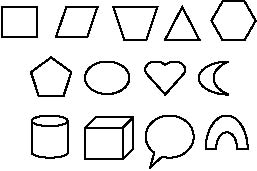
\includegraphics[scale=0.5]{symbolSet.PNG} 
		\caption[The Symbol Set] {The symbol set}   \label{fig:symbolSet}
	 \end{figure}
	
To demonstrate the change in accuracy is due to the enhanced swarm optimization algorithm we tested the recognition system using two sets of features. Firstly, we tested recognition accuracy of shapes in the data set with both algorithms (\textsl{AlgS1} and \textsl{AlgS2}) using the whole feature set. The second experiment was tested on both algorithm but only using half the feature set. Both experiments were compared with the original sketch recognition system presented in \cite{mypaper}. 

Figures \ref{exp2} and \ref{exp1} show the recognition rate of each algorithm using the full feature set and half the features set respectively. The figures compares between the result that can be obtained by system in \cite{mypaper} and modifying the system using Enhanced PSO. The results show that the enhanced swarm optimization algorithm improves the segmentation of the system which leads to an increase in the recognition rate of the whole system by an average of $1.5\%$.  The increase in recognition rate is consistent in all swarm algorithms and in both experiments.   
    \begin{figure}
  \centering
  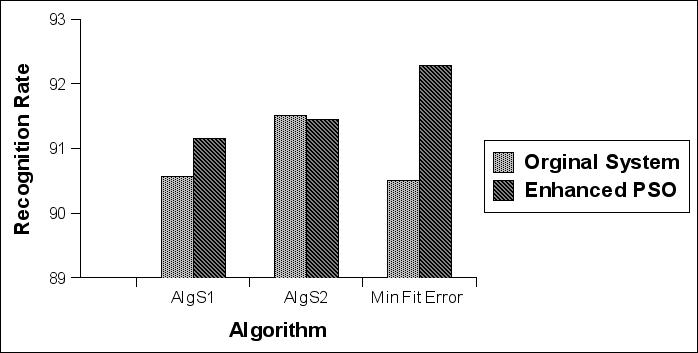
\includegraphics[width=3.3in]{Experiment92.jpg}
  \caption[Recognition accuracy]%
  {The chart compares between recognition rate of the full feature set on both the original system presented in \cite{mypaper} and Enhanced PSO. The results shows that Enhanced PSO increases the performance over the original system. }
   \label{exp2}
\end{figure}
\begin{figure}
  \centering
  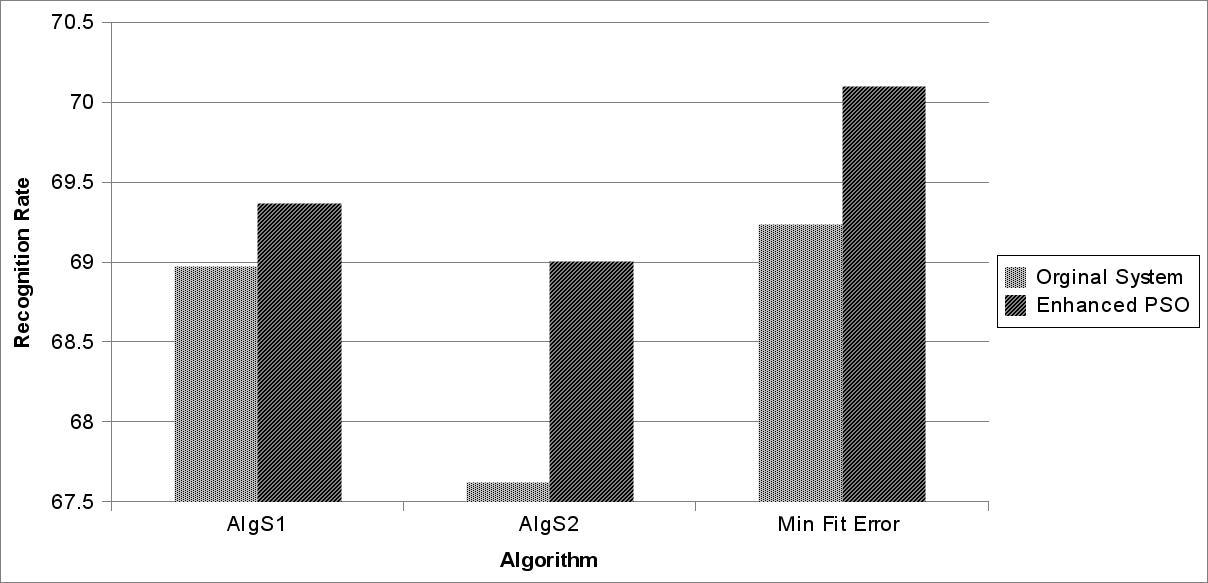
\includegraphics[width=3.3in]{Experiment68.jpg}
  \caption[Recognition accuracy]%
  {The chart compares between recognition rate of half the feature set on both the original system presented in \cite{mypaper} and Enhanced PSO. The results shows that Enhanced PSO increase the recognition rate. }
   \label{exp1}
\end{figure}

 
  
\section{Conclusion }
 \label{ConclusionandFutureWork}


This paper used an Enhanced-PSO  to modify a new sketch recognition using DPSO represented in \cite{mypaper}. Results show that enhancing the solutions that the \textit{PSO} in general generates an optimized stroke segmentation which improves the final recognition rate.  The final recognition improved by modifying the particle optimization algorithm without depending on the higher level features. The experiments evaluated two \textit{DPSO} different segmentation algorithms (AlgS1 and AlgS2) on simple presentation set dataset. Results show that the enhanced PSO algorithm improves the segmentation on both algorithms which achieves better segmentation and final accuracy. The results proved that the Enhancement made on the PSO improves the efficiency of the Basic PSO algorithm without being dependable on special objective function or application. The system achieved an average overall improvement of more than 1\% over Basic PSO.  

 For the future work, it is suggested that we continue to improve both the enhanced PSO segmentation algorithm. Also, a possible extension of this research is to improve the recognition algorithm of the Sketch Recognition system. Other area of enhancements is the features extraction methods. Introducing more spatial and geometrical features is believed to improve classifications. 

\bibliographystyle{IEEEbib}
\bibliography{../../../neededfiles/Bibliographies/Mybibliography}

\end{document}

